\documentclass[11pt]{article}

% Make margins smaller
\usepackage[top=0.65in, bottom=0.65in, left=0.6in, right=0.6in]{geometry}
% more advanced mathematical symbols
\usepackage{amsfonts}
\usepackage{amssymb}
\usepackage{amsmath}
\usepackage{bm}
\usepackage{bold-extra} % bold texttt
\usepackage{graphicx}
\usepackage{enumerate}
\usepackage[font=small,labelfont=bf]{caption} % Required for specifying captions to tables and figures
\usepackage{pgfgantt} % gantt chart!
\usepackage{titling}

\graphicspath{ {./images/} }

% so that we can skip any number of items in an enumeration
\makeatletter
\newcommand{\skipitems}[1]{%
  \addtocounter{\@enumctr}{#1}%
}
\makeatother

\begin{document}

\title{\textbf{Virtual Reality Summative}}
\date{for 15th March 2019}
\author{Bradley Mackey}
\maketitle


\section*{Question Remarks}

\begin{enumerate}
\item \texttt{get\_sanitized\_imu\_data()} returns the corrected data readings from the csv file, returning a 2D array of data rows. \texttt{reading\_to\_qtrn(reading,prev\_sample\_time)} computes a quaternion $(a,b,c,d)$ from a given input gyroscope reading and previous sample time, such that the delta rotation is calculated correctly. \texttt{euler\_to\_qtrn(axis, angle)} takes an axis of rotation $(x,y,z)$ and angle $\theta$ in radians, returning a quaternion $(a,b,c,d)$.  \texttt{qtrn\_to\_euler(qtrn)} takes a quaternion $(a,b,c,d)$ and returns a tuple of the rotation axis and angle rotation this quaternion represents $((x,y,z),\theta)$. \texttt{qtrn\_conj(qtrn)} takes a quaternion $(a,b,c,d)$ and returns its conjugate, $(a,-b,-c,-d)$. \texttt{qtrn\_mult(qtrn\_1, qtrn\_2)} computes the product of 2 quaternions.

% NO REPORT REQUIRED FOR QUESTION #2
\skipitems{1} 


\item Try a few different alpha values (e.g., 0.01, 0.1, ...), investigate and comment on their effect on drift compensation in your report (7 marks)
\item Try a few different alpha values (e.g., 0.01, 0.1, ...), investigate and comment on their effect on drift compensation in your report (5 marks).
\end{enumerate}

\section*{Visualisations}

\begin{figure}[htp]

\centering
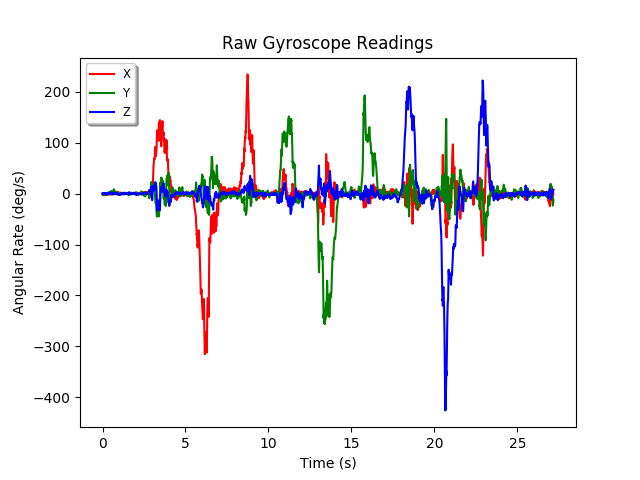
\includegraphics[width=.32\textwidth]{gyro-unaltered}\hfill
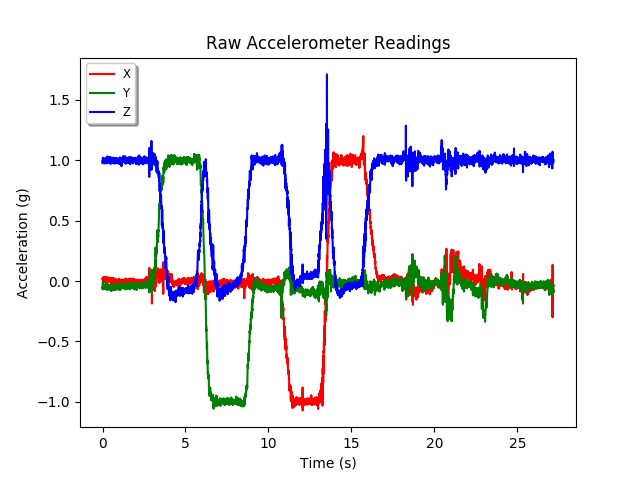
\includegraphics[width=.32\textwidth]{acc-unaltered}\hfill
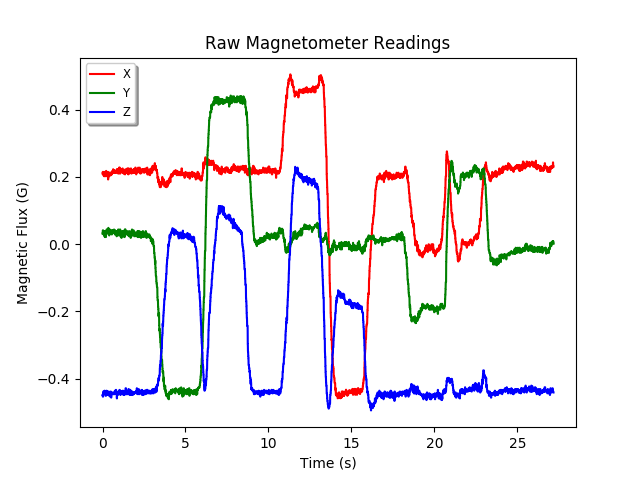
\includegraphics[width=.32\textwidth]{mag-unaltered}

\caption{Raw sensor readings from the IMU.}
\label{fig:figure3}

\end{figure}



\end{document}